La \bnf constate le besoin d'automatisation pour traiter les volumétries
croissantes des collections numérisées, en outre caractérisées par une
variété considérable, et elle relève les tensions se jouant dans le traitement en
masse de données hétérogènes.

\begin{kwote}

"De plus en plus confrontées à des niveaux de volumétrie et de vélocité
typiques des mégadonnées (big data), les collections numériques de la
\bnf, qui occupent aujourd'hui environ six pétaoctets, sont caractérisées
par une variété considérable. Documents numérisés, tels que par exemple
les livres et manuscrits consultables dans Gallica --- la bibliothèque
numérique de la \bnf ---~; documents nativement numériques comme les
œuvres d'art vidéo, les logiciels, les bases de données, les archives de
l'Internet~; métadonnées bibliographiques et données d'autorité
décrivant les personnes, lieux, organisations, concepts\ldots{} autant
d'ensembles de données diverses en termes de structures, formats,
qualité, contextes de production, fonctions et contenus. Ces ensembles
ont des histoires différentes, issues des changements des supports et
des multiples strates de pratiques documentaires accumulées au fil du
temps. Leur hétérogénéité exige des traitements spécifiques et par
conséquent des compétences et des méthodes particulières, aussi bien
pour les conserver ou les communiquer que pour les analyser (cf
Moiraghi, 2017). Cette hétérogénéité des données, qui découle de
l'amplitude chronologique et de la vocation à l'encyclopédisme
caractéristiques des bibliothèques nationales, s'ajoute à
l'accroissement de la quantité des données en entrée et à l'accélération
conséquente des temps de traitement. La tendance traditionnelle des
bibliothèques à la systématisation des procédures doit dès lors trouver
son équilibre face à la spécificité des données mais aussi des questions
scientifiques propres aux projets de recherche qui les
exploitent".\footcite[p.6]{bermes_patrimoine_2020}  
\end{kwote}

L'état de l'art montre une convergence vers l'utilisation de
l'intelligence artificielle pour traiter efficacement des corpus de
données de plus en plus vastes et complexes. Cette systématisation doit
cependant être équilibrée par une compréhension fine des contextes
locaux et spécifiques des données, afin de garantir la pertinence et
l'efficacité des outils développés.

Les explorations autour du traitement du patrimoine numérique menées à
la \bnf\footnote{\cite{bermes_patrimoine_2020}, \cite{beaudouin_cartographie_2017}, \cite{michez_gallicapix_2021}, \cite{bouchard_presentation_2017}},
en rapport étroit avec des projets de recherche en \hn, illustrent bien
cette tension. Ces projets ont porté sur des ensembles de données
balisés et spécifiques (tel que les sources documentaires numérisées
autour de la guerre 14-18, les publicités de 1910 à 1920, illustrations
du magazine de mode Vogue de 1920 à 1940 ou encore illustrations de
papier peint\footnote{\cite{beaudouin_cartographie_2017}, \cite{michez_gallicapix_2021}}). L'absence de
passage à l'échelle est significatif des difficultés d'un traitement et
d'un enrichissement systématique et standardisé de très grands volumes de données très
hétérogènes. Ainsi, chacun des projets reposait sur des méthodes et des
techniques différentes en raison de la nature des données explorées et
des finalités scientifiques propres à chaque projet.

Cependant des leçons ont été tirées~: les résultats découlent d'un
travail collectif et interdisciplinaire, et se sont appuyés sur des
méthodes standardisées, par exemple pour l'extraction des données et
métadonnées via des \apis\footcite[p.7]{bermes_patrimoine_2020}. Ces
premières applications de l'\ia ont démontré la nécessite de garantir la
reproductibilité des méthodes et d'adopter des normes pouvant mettre en
œuvre un cadre technique interopérable afin de faciliter la
collaboration à plusieurs échelles~: entre les projets de recherche d'un
part, et d'autre part entre les disciplines et les corps de métier
(notamment entre les chercheur.ses et les professionnels des
bibliothèques).

Le projet \gaga\footnote{https://gallicorpora.github.io/} --
bénéficiant de l'appui du DataLab de la \bnf -- se détache néanmoins dans
le paysage des projets estampillés \bnf, car il aspire à s'éloigner le
plus possible de son corpus, voulant concilier reproductibilité des
résultats sur des données diverses et applicabilité à un large corpus
issu des collections numérisées de la Bibliothèque Nationale. Il
illustre en outre les problématiques susmentionnées~: l'inscription dans
un dialogue interdisciplinaire et dans des pratiques normalisées.
L'ambition du projet porte sur le développement d'une chaîne de
traitement automatisée pour la transcription et l'annotation des documents textuels historiques, en diachronie longue, en
partant de leurs numérisations disponibles sur le portail Gallica,
créant ainsi des corpus enrichis, et facilitant leur exploitation et
leur valorisation. En effet les besoins des institution se déplacent de la transcription des textes à leur encodage sémantique automatique en \xml-\tei, afin d'offrir
utilisateur.rices de bibliothèques numériques de nouvelles options pour la
fouille de données. Le projet \gaga s'inscrit dans cette
dynamique, en exploitant le riche corpus de la \bnf, qui met à disposition 193 265
manuscrits, dont 52 188 précédent 1800, et 1 182 471 livres imprimés,
dont 160 335 précédent 1800\footcite{sagot_gallicorpor_2022}.

\begin{kwote}  
``Le nouveau défi à relever aujourd'hui est de transformer ces
numérisations en des ressources enrichies, qui augmentent le texte
extrait et repérable avec de la métadonnée et de l'analyse. Le texte
brut et non annoté ne suffit plus pour la recherche en informatique
appliquée aux documents historiques. De là vient l'impulsion pour le
projet \gaga. Le projet envisage la mise en place d'un pipeline
qui saisit un document numérisé depuis le portail Gallica et renvoie une
ressource numérique très enrichie. En plus d'une description du texte
repérable, la ressource présentera les données structurelles portant sur
la mise en page, ainsi qu'une analyse linguistique du texte extrait et
des métadonnées portant sur le document physique et le fac-similé
numérique''.\footcite{christensen_gallicorpor_2022}.
\end{kwote}

En outre, le but sous-jacent du projet est de produire un prototype qui
pourrait servir d'exemple de chaîne d'acquisition
numérique pour les institutions
patrimoniales. Par conséquent, ce projet se propose aussi d'être une
preuve de concept d'un \emph{modus operandi} pour l'extraction et
l'annotation de textes très divers, créant une sorte de \textit{pipeline} ultime. Mais avant tout, la chaîne de traitement est destinée à être applicable
à un large corpus de documents mis à disposition par la \bnf. Les
documents du corpus visé proviennent de différentes époques (du \textsc{xv}\ieme au
\textsc{xviii}\ieme siècle) et présentent une grande diversité de mises en page, de
langues (ancien français, moyen français, français classique), et de
supports (manuscrits, imprimés). L'hétérogénéité des sources est censée
faire preuve de faisabilité, et vérifier le potentiel de la méthode
élaborée. Elle vise à prouver que le concept d'une chaîne de traitement
généraliste peut être concrètement appliquée.

\gaga expose ainsi la plupart des questionnements et défis
tenant au montage d'une chaîne de traitement unifiée applicable à une
grande diversité de données. Les choix technologiques, tels que
l'adoption de formats ouverts et interopérables, la prise en compte de
la diversité des modes d'acquisition des données et la spécialisation
des modèles d'\ia, sont au cœur de ces enjeux. Par ailleurs, la question
de l'ouverture des corpus annotés, essentielle pour l'apprentissage
machine, est également un axe d'analyse à considérer.

                \hypertarget{formats-standards}{\section{%
                Formats standards}\label{formats-standards}}
                    
L'astronomie est issue d'une tradition continue vieille de près de 4000
ans qui transcende les cultures et les langues. Les théories, les
savoirs, les méthodes, au gré de leur diffusion, se mélangent aux
pratiques autochtones pour servir les usages locaux, qui bien souvent
renforcent des dynamiques de pouvoir en place, que ce dernier soit
politique ou religieux. Les sciences astrales revêtent ainsi une
importance culturelle majeure.

Une étude approfondie des sources révèle les processus par lesquels les
connaissances se sont enrichies et transformées au contact de
différentes cultures. Leur examen permet en outre de souligner les
spécificités et les innovations de chaque tradition, tout en montrant
les interconnexions et les influences réciproques qui ont façonné
l'évolution de l'astronomie. Les schémas de circulation sont dans de
nombreux cas de très grande portée géographique, chronologique et
culturelle. Ils relient des contextes de production de connaissances à
l'échelle afro-eurasienne et sur des périodes de siècles voire de
millénaires. La trace de ces transmission supporte une vision connectée
et globale de l'histoire des cultures et du savoir.

La grande diversité des sources et des approches possibles rend
cependant difficile une approche globale. À ce titre, il est important
de cibler un objet d'étude : \eida se focalise ainsi essentiellement dans
la transmission de la tradition ptoléméenne, et le corpus se compose
donc de ressources manuscrites et imprimées relevant de cette tradition.

\hypertarget{ptolemee-modele-et-transmission}{%
\subsection{Ptolémée : modèle et
transmission}\label{ptolemee-modele-et-transmission}}

Ptolémée tient une place proéminente dans l'histoire de l'astronomie et
des mathématiques. Son nom reste associé à la conception d'un système
astronomique qui plaçait la Terre immobile au centre du monde, et dont
la mise en question, de Copernic à Newton, a commandé la révolution
scientifique.

Dans sa \emph{Syntaxe mathématique}, plus connue sous le titre
d'\emph{Almageste}, et dont la dernière observation consignée date de
141, il expose l'ensemble des connaissances astronomiques de son époque.
Notamment il perfectionne le modèle élaboré par Hipparque, à qui il
emprunte la découverte de l'excentricité des trajectoires apparentes du
Soleil et de la Lune par rapport à la Terre, et l'idée de composer ces
trajectoires à l'aide de deux mouvements distincts. Il élabore un
système géocentrique au moyen d'un ensemble complexe de trajectoires
circulaires des objets pris dans un mouvement uniforme : les déférents,
autour de la Terre, et les épicycles, dont les centres parcourent les
déférents\footcite{lequeux_systeme_nodate}.

En effet, les sociétés anciennes attendent des
corps astraux (soleil, lune, planètes et étoiles) un mouvement uniforme
et le plus ``parfait'' possible, c'est-à-dire un cercle. Pourtant la
trajectoire de ces corps, observée empiriquement, n'est pas circulaire.
Le modèle de Ptolémée explique ces imperfections en postulant que les
mouvement apparemment irréguliers sont dû à cette fameuse combinaison de
plusieurs trajectoires circulaires régulières vues depuis la Terre,
point statique. Les planètes se déplacent à vitesse uniforme sur un
cercle (l'épicycle) dont le centre se déplace à vitesse uniforme sur un
cercle coplanaire (le déférent), dont la Terre est le centre.

En plus de la description du mouvement des astres, Ptolémée dresse dans
l'\emph{Almageste} des tables établissant les positions de la lune et
prévoyant les périodes et les caractéristiques des éclipses avec une
précision inédite\footcite{raymond_jones_ptolemy_2024}, un catalogue des étoiles, un traité
complet de trigonométrie plane et sphérique et une description des
instruments nécessaires à un grand observatoire.

L'œuvre de Ptolémée fera référence, et en tant que synthèse des
connaissances astronomiques antérieures, sa transmission correspond
à celle de la vision des pratiques de l'astronomie grecque à son apogée,
et sa diffusion façonnera la production astronomique ancienne pendant
près de treize siècles. D'ailleurs le nom d'Almageste date de la
transmission par les civilisations arabes à l'occident.

En effet, lors de la chute de l'Empire Romain d'occident, la majeure
partie des ouvrages antiques sont perdus et la science occidentale
stagnera jusqu'au \textsc{xii}\ieme siècle. Elle continuera cependant à progresser
ailleurs : notamment dans le monde arabe et musulman. Dès le \textsc{viii}\ieme et
\textsc{ix}\ieme siècle, les Arabes vont traduire dans leur langue la plupart des
grands textes scientifiques de l'Antiquité, en particulier les œuvres
d'Aristote et l'\emph{Almageste} de Ptolémée. Sans remettre en cause le
géocentrisme et le système de Ptolémée, ils le perfectionnent et
l'amènent à un très grand degré de précision. Nécessaire à la stricte
observation des règles de l'islam, l'astronomie arabe se développe et se
diffuse, grâce aux travaux d'al-Biruni, al-Hazen ou al-Sufi\footcite{noauthor_monde_nodate}.

À partir du \textsc{xi}\ieme et surtout du \textsc{xii}\ieme siècle, au fil des conquêtes des
occidentaux en Espagne et en Sicile, les textes grecques sont traduits
en latin via la traduction arabe. La transmission des savoirs
gréco-arabes -- notamment les traductions arabo-latines de
l'\emph{Almageste} et du Livre des étoiles fixes d'al-Sufi -- ouvre la
voie à un renouveau scientifique dans l'Occident chrétien, permettant
ainsi l'essor des grandes universités européennes de l'époque (Paris,
Oxford, Bologne, etc). On redécouvre les modèles d'Aristote et de
Ptolémée en les adaptant aux conceptions chrétiennes\footcite[``Le
  système géocentrique devient le modèle astronomique et théologique de
  l'Église, qui ne remet pas en cause la sphéricité de la Terre''][]{noauthor_monde_nodate}.

Avant l'avènement de l'astronomie grecque, les Babyloniens, dès le premier
millénaire \jc, utilisaient des calculs arithmétiques pour prévoir
la position des planètes. Ces théories ont voyagé jusqu'en Perse et en
Inde, où elles ont été adaptées et combinées à des méthodes autochtones.
Les théories grecques de l'époque de Ptolémée et de son prédécesseur
Hipparque sont également parvenues jusqu'en Inde, créant un matériel
complexe dont les influences sont difficiles à démêler. Parmi les
pratiques empruntées aux théories grecques, on relève l'emploi de termes
-- par exemple le titre du canon \emph{Romaka Siddhanta} datant du début
du \textsc{v}\ieme et qui marque les origines de la science astronomique sanskrite --
ainsi que des modèles épicycliques et des méthodes de calculs requérant
des paramètres numériques hérités d'Hipparque\footnote{\cite[p.6-7]{mercier_studies_2004} in \cite[p.15]{albouy_mediation_2019}}.

La tradition chinoise se développe de manière relativement indépendante
et les échanges ne débutent qu'autour de 200 \jc. Elle se distingue
de celle des Grecs par un intérêt plus marqué pour la prédiction
d'événements singuliers plutôt que pour les théories cosmologiques
cherchant l'établissement d'un modèle d'organisation du ciel. En effet,
en Chine impériale, l'astronomie a une fonction politique. L'empereur
est considéré comme le Fils du Ciel et ainsi la régulation du
calendrier, ou bien le succès (ou l'échec) de ses astronomes à prédire
une éclipse, se reflétaient positivement ou négativement sur lui.
L'inclusion croissante des diagrammes dans les traités après les
missions jésuites à partir du \textsc{xvi}\ieme siècle révèle l'influence des
pratiques d'Europe de l'ouest.

Pour conclure, l'\emph{Almageste} se présente donc comme une sorte
d'encyclopédie des connaissances d'une époque qui s'est enrichie avec le
temps au point de rendre difficile l'appréciation de son état originel.
Œuvre sans cesse recopiée au cours des siècles, passant du grec à
l'arabe puis au latin, transmise à travers tout le bassin méditerranéen
et dominant le \ma occidental après avoir conquis l'Islām, chaque
traduction et chaque copie de l'Almageste n'ont pas seulement transmis
son contenu, mais l'ont aussi adapté et enrichi en fonction des
contextes culturels et scientifiques de chaque époque. L'œuvre
ptoléméenne a servi de base à de nombreux commentaires et traités,
intégrant progressivement des éléments de connaissance issus de diverses
traditions scientifiques, et illustrant ainsi l'interconnexion des
savoirs à travers les civilisations.

\begin{kwote}
``Certains indices dans les manuscrits révèlent les emprunts
intellectuels qui s'opèrent au fur et à mesure des copies ; les méthodes
de calcul, le tracé des diagrammes, la mise en page des tables, la
structuration des textes techniques, la mention d'auteurs antérieurs, la
réutilisation de paramètres astronomiques ou même la récurrence de
certaines erreurs sont autant de signes qui témoignent des échanges
culturels qui ont façonné la pratique de l'astronomie.''\footcite[p.14]{albouy_mediation_2019}
\end{kwote}

Comme l'entend \citeauthor{albouy_mediation_2019}, les diagrammes font partie des révélateurs des
échanges intellectuels.

\hypertarget{le-diagramme-vecteur-de-connaissances}{%
\subsection{Le diagramme vecteur de
connaissances}\label{le-diagramme-vecteur-de-connaissances}}

L'historiographie et l'histoire des sciences n'échappent pas au récent
``visual digital turn''\footcite[``Digital humanities research has
  focused primarily on the analysis of texts. This emphasis stems from
  the availability of technology to study digitized text. Optical
  character recognition allows researchers to use keywords to search and
  analyze digitized texts. However, archives of digitized sources also
  contain large numbers of images.''][]{wevers_visual_2020} général des
humanités, montrant à quel point la production et la diffusion du savoir
croisent les représentations visuelles rendant compte de ces
connaissance. De fait, on ne s'intéresse plus seulement au texte. Or les
astronomes, au fil de l'histoire, ont eu recours à un grande diversité
de matériaux. Les sources primaires sont constituées par des instruments
et des écrits, ces derniers eux-même hétérogènes. Dans les traités
anciens, on trouve des descriptions détaillées, des propositions
mathématiques, des tables de calcul, et des diagrammes illustrant
souvent le texte qu'ils accompagnent. Les sources primaires peuvent en
outre être enrichies de commentaires et de gloses, prose ou
illustrations, témoignant de la manière dont les connaissances ont été
transmises et interprétées. Elles révèlent également les méthodes
pédagogiques employées pour enseigner ces savoirs.

Au cœur de cette diversité, le diagramme, objet hybride pour deux
raisons : il combine un contenu géométrique (des lignes, arcs et
cercles) et des labels, et il entretient un lien (plus ou moins étroit)
avec le texte qui l'accompagne.

En tant que structure de pensée, la figuration géométrique -- une forme
de création de modèles associée à l'élaboration et à la résolution de
problèmes dans divers domaines de la pensée humaine liés au calcul
abstrait et à la modélisation des idées -- est aussi ancienne que
presque toute autre forme d'enregistrement des pensées et des idées. Des
diagrammes utilisés pour calculer la superficie de parcelles et de
terres apparaissent dans le Papyrus mathématique Rhind, la source la
plus importante qui subsiste pour l'histoire des mathématiques dans
l'Égypte ancienne\footcite[p.6]{safran_diagram_2022}. Instruments
de pensée et de démonstration, ils servent non seulement à transmettre
le savoir mais aussi à le produire. Et dans un étrange mouvement
métaréflexif, ils permettent aux historien.nes des sciences de produire la
connaissance sur ces anciennes traditions heuristiques et leur
transmission.

Les diagrammes sont, pour les astronomes, le support d'une pratique
scientifique, et sont ainsi révélateurs de leurs méthodes, de leur
contexte d'exercice et de leur conception de leur discipline. Ils
revêtent des rôles et des aspects différents, permettant d'identifier
des modes diagrammatiques\footnote{La ``diagrammatisation'' désigne
  assez largement l'investissement des acteurs dans la complexification
  des représentations visuelles des propositions scientifiques présentes
  dans les traités.} spécifiques d'un lieu ou d'une époque, et traçant
des lignes de diffusion des pratiques et des savoirs.

Au \ma, trois grandes cultures coexistent en Eurasie : les
cultures byzantine, islamique, et d'Europe occidentale. Elles
connaissent des évolutions différentes en termes linguistiques et
religieux ; cette diversité est vraie également pour les usages auxquels
les diagrammes astronomiques étaient destinés, pour les domaines dans
lesquels ils étaient reconnus comme des instruments de pédagogie et des
vecteurs de pensée, ainsi que pour la place accordée à la culture
visuelle plus généralement et aux modes de représentation
diagrammatiques. Pourtant cette coexistence donne lieu à des échanges
intellectuels, artistiques, diplomatiques et commerciaux. Les
traductions d'œuvres savantes, les transferts de manuscrits illustrent
la porosité des frontières du savoir et de l'interdépendance des
cultures. Les diagrammes astronomiques sont à ce titre témoins des
chemins de diffusion des connaissance et des pratiques des sciences.

\emph{Comment ces diagrammes parlent-ils aux historien.nes ?}

Les diagrammes peuvent être étudiés intrinsèquement (quelles conventions
gouvernaient le langage visuel, quelle fonction assumaient-ils ?) ou
extrinsèquement (pour comprendre la transmission de ces traditions et
ces pratiques entre l'Europe et l'Asie, en passant pas la péninsule
arabique).

On pourrait penser que les formes et éléments visuels
utilisés pour une démonstration géométrique soient universels, qu'ils
restent les mêmes quelle que soit la date et la langue de l'explication
textuelle, le grec, l'arabe ou le latin\ldots{} Et pourtant le contexte
géographique, temporel, et les aspects matériels liés aux technologies
d'inscription changent profondément le fonctionnement et les objectifs des diagrammes,
leurs objectifs.

L'évolution des conventions graphiques en sont un exemple frappant. Par
exemple, l'axe vertical de la Terre, bien que représenté à plat sur la
page, fut conventionnellement compris comme un axe perpendiculaire à la
coupe du globe. Au fil du temps, de nouvelles conventions graphiques ont
été adoptées, et pour les lecteurs d'aujourd'hui on représenterait
sûrement le globe terrestre avec sa profondeur pour expliciter la
représentation. Citons en outre la représentation des phases lunaires,
qui a connu une évolution concernant l'association des couleurs claire
et sombre à la pleine lune et à la nouvelle lune. Si aujourd'hui on
associerait plutôt la pleine lune à un aplat de couleur claire et la
nouvelle lune à une couleur sombre, les manuscrits médiévaux byzantins
adoptent le référentiel contraire.

De même, le rôle du diagrammes est fluctuant, et va au delà du simple
support démonstratif au service du texte. Par exemple ceux des
\emph{Traités logiques} d'Aristote ont probablement circulé
indépendamment du texte, même si tout indique que les écrits les
appelaient dès le départ. Cela souligne la distinction entre le
diagramme en tant qu'objet de démonstration et de discussion complétant
une proposition d'un côté, et le diagramme en tant qu'accompagnement des
textes scolaires, qui aide à la compréhension de l'autre\footcite[p.5]{safran_diagram_2022}. Le
diagramme peut ainsi constituer la preuve et le support d'une
réinterprétation de la proposition textuelle.

Par-dessus tout, les transformations subies au fil des copies et des
réceptions sont éloquentes pour les chercheurs. Bien que les diagrammes
soient initialement conçus pour clarifier et expliquer une proposition textuelle, ils peuvent
parfois être des vecteurs de confusion (ou d'innovation). Le même diagramme d'une même
œuvre soumis à un processus constant de transformation par les scribes,
les artistes ou les lecteurs/commentateurs. 

La recherche des erreurs
transmises a ainsi un intérêt philologique important. Les cas de
méprises et les malentendus sont peut-être plus nombreux que les cas de
compréhension fidèle lors de la traversée des frontières géographiques,
culturelles, religieuses et/ou linguistiques, et l'étude des erreurs et modifications
révèle leurs aspects heuristiques, autant qu'il peut amener à
l'établissement d'un stemma\footcite{raynaud_building_2014}.

L'importance des diagrammes dans les transmissions est illustrée par l'exemple des diagrammes attribués à al-Ḥajjāj, en lien avec la transmission arabe des \emph{Éléments} d'Euclide. Bien que la traduction originale d'al-Ḥajjāj soit perdue, les diagrammes retrouvés dans divers manuscrits montrent qu'il utilisait parfois des schémas différents de ceux adoptés dans la tradition arabe ultérieure. Ces diagrammes ont probablement joué un rôle clé dans l'élaboration d'une version alternative de la géométrie euclidienne, influençant ainsi la transmission vers l'Europe via les traductions latines et hébraïques\footcite{de_young_editing_2014}.

Ainsi, au travers des variations, similarités et évolutions des
diagrammes, les historien.nes peuvent reconstruire les pratiques
scientifiques des astronomes et comprendre les contextes culturels et
sociaux dans lesquels elles s'inscrivaient. De telles études permettent
aussi de tracer la circulation des sources dans le monde entre les
différentes cultures et de comprendre comment celle-ci s'approprient le
contenu. En somme, l'évaluation de phénomènes diagrammatiques
indéniablement disparates à travers des géographies éloignées permet
d'identifier des modalités d'échanges culturels et leur impact sur la
construction du savoir scientifique.

Les travaux antérieurs sur l'illustration scientifique se concentrent
essentiellement sur des types spécifiques de diagrammes, situés dans des
contextes déterminés chronologiquement et culturellement. Un exemple de
ce paradigme est le projet précédent ALFA, qui porte sur les diagrammes
de tradition alfonsine médiévaux un regard eurocentré. Cependant, à
l'aune des remarques précédentes, il devient pressant de dépasser cette
perspective centripète en étendant la portée géographique et temporelle
des projets ; ambition rendue possible par la disponibilité des sources
primaires en ligne, permettant la construction de bases de données
d'images de grande envergure. Ainsi peut être mise en œuvre une analyse
plus inclusive et diversifiée des sources iconographiques -- notamment
les diagrammes\footcite{husson_eida_2022}.

Comme le dit Jeffrey F. Hamburger dans un plaidoyer pour une étude
comparative des diagrammes astronomique : ``Diagrames can thus be seen
not as embodiements of eternal truths, but, rather, as culturally
embedded objects''\footcite[p.7]{safran_diagram_2022}.

\begin{kwote}
``(\ldots) to be effective, a cross-cultural comparison of diagrammatic
traditions must look beyond the prima facies appearence of the diagrams
under consideration to their underlying operations and the patterns of
thoughts that they both codified and were intended to
inculcate.''\footcite[p.3]{safran_diagram_2022}
\end{kwote}         

Les interrogations soulevées par le projet \eida se déclinent donc comme
suit : analyser l'articulation entre les fonctions documentaires et
épistémiques des diagrammes au sein de l'histoire des pratiques
astronomiques, interroger l'importance des diagrammes dans la
construction et la transmission des connaissances scientifiques, et
enfin identifier des schémas récurrents dans les modalités de
circulation de ces diagrammes. S'appuyant sur ces analyses, les
chercheurs pourront à leur tour tracer des lignes : au sens figuré
construire ``a web of connections linking the points represented by the
individual contributions together into a larger pattern''\footcite[p.10]{safran_diagram_2022} ; et
au sens propre, cette vision globale sur la vie des images et des œuvres
pouvant permettre l'établissement d'éditions critiques normalisées.
                    
                 \hypertarget{specialisation-modeles}{%
                \section{La spécialisation des modèles}\label{specialisation-modeles}}
                L'objectif commun des deux projets parallèles \eida et \vhs est de
proposer une nouvelle approche de l'étude historique de la circulation
des connaissances scientifiques basée sur de nouvelles méthodes
d'analyse des illustrations. Le développement d'outils numériques pour
l'étude des diagrammes astronomiques -- notamment l'application de
techniques de vision artificielle -- permet d'automatiser une série de
traitements et ainsi de faciliter leur analyse et exploitation. Ces
outils ont pour objectif de réduire les étapes manuelles de fouille et
d'annotation, optimisant ainsi l'efficacité des recherches, et
permettant également de poser un regard neuf sur les objets.

\hypertarget{des-outils-dexploration-et-danalyse-dun-large-corpus}{%
\subsection{Des outils d'exploration et d'analyse d'un large
corpus}\label{des-outils-dexploration-et-danalyse-dun-large-corpus}}

L'ouverture des données met à disposition des chercheur.ses des documents
variés en masse, ce qui a des conséquences profondes sur les
méthodologies de la recherche scientifique.


\subsubsection{EIDA/VHS~: des préoccupations
proches}

\begin{kwote}
"There are tens of thousands of manuscripts and early prints in Latin,
Greek, Arabic/Persian, Sanskrit and Chinese extent today which include
different types of texts, numerical tables and diagrams. Indeed,
astronomers made extensive and refined uses of non-discursive modes of
expression, such as numerical tables and diagrams, in their practice.
The analysis of the precise interactions of the different discursive
(textual) and non-discursive (tables and diagrams) elements that compose
these documents is key to our understanding of a history of astral
sciences that goes beyond the ``surface'' of doctrines and astronomical
models as presented in texts and opens up the potential of the history
of astral sciences for global history".\footcite{husson_eida_2022}.
\end{kwote}       

L'abondance d'archives et de documentation laissées par les astronomes
prémodernes et modernes posent un défi majeur en termes d'exploitation
en raison de la difficulté à mener des études à cette échelle.
Cependant, le traitement par \ia est
prometteur, pour accélérer l'exploration des corpus et interroger les
modalités de circulation des savoirs scientifiques, ainsi que le rôle et
la place de l'image dans la transmission des connaissances. Le but est
de pouvoir donner du sens aux images en évitant au maximum les étapes
manuelles d'annotation. Pour ce faire, \eida et \vhs développent des
méthodes d'apprentissage non ou faiblement supervisées permettant
d'effectuer des recherches automatiques à grande échelle dans des corpus
d'envergure. L'utilisation du \dl est centrale pour accomplir
divers traitements analytiques qui accompagnent l'étude des modalités
d'évolution et de transformation des images dans des corpus
scientifiques illustrés.

La collaboration \eida / \vhs a pour but de créer un outil à la fois
polyvalent (une sorte de couteau suisse) et précis, c'est pourquoi il
est nécessaire de différencier et paralléliser les tâches en raison des
finalités spécifiques de chaque projet. Cependant, une base commune
repose sur deux aspects essentiels~: la constitution des corpus
numérisés et l'extraction automatique de leurs illustrations dans une
base de données d'images au format \iiif, dotée d'une interface numérique
de consultation et d'annotation partagée.

\hypertarget{divergences-et-finalites}{%
\subsubsection{Divergences et finalités}\label{divergences-et-finalites}}

Les objectifs de \eida et \vhs sont proches mais des divergences
apparaissent en raison de la nature distincte des corpus, ce qui
entraîne des finalités différentes dans la chaîne de traitement.

Côté \vhs la vision artificielle sert l'analyse d'un large corpus
scientifique illustré du \ma et de la période moderne, ne se
limitant pas aux sciences astronomiques. La méthodologie adoptée
consiste essentiellement à rechercher et identifier (dans un corpus de
manuscrits témoins d'un même travail) les illustrations qui se
correspondent. Cette tâche est ardue pour les ensembles de manuscrits
contenant parfois des centaines d'illustrations, séparés par de
nombreuses copies perdues, s'étalant sur des siècles, et qui ont pu être
complètement réorganisés et fortement modifiés pour s'adapter à de
nouvelles connaissances ou croyances\footcite[``Most research on the
  automatic analysis of manuscripts and particularly their alignment,
  also known as collation, has focused on text. However, illustrations
  are a crucial part of some documents, hinting the copyist values,
  knowledge and beliefs and are thus of major interest to historians.
  One might naively think that these illustrations are much easier to
  align than text and that a specialist can identify them in a matter of
  seconds. This is only true in the simplest of cases, where the order
  of the illustrations is preserved and their content relatively
  similar. In harder cases however, the task becomes daunting and is one
  of the important limiting factor for a large scale analysis.''][p.1]{kaoua_image_2021}.

\begin{kwote}
"{[}N{]}otre approche consiste à concevoir des méthodes basées sur la
vision artificielle pour détecter les similitudes iconographiques
(c'est-à-dire des images qui ont été copiées ou partiellement inspirées
les unes des autres) et textuelles (des images qui décrivent un contenu
textuel similaire mais qui peuvent être visuellement différentes) entre
des illustrations dans de grands corpus. L'un des principaux objectifs
est d'obtenir ces associations automatiquement, en s'appuyant le moins
possible sur les annotations d'experts, qui sont coûteuses et
compliquées à obtenir. Nous faisons l'hypothèse que de telles méthodes
d'analyse permettront d'effectuer beaucoup plus efficacement des
comparaisons et des rapprochements pertinents entre images car elles
fourniront, d'une part, de nouveaux regroupements d'images en fonction
de leur contenu et des textes qu'elles illustrent et, d'autre part, des
distinctions fines entre les différentes modalités de représentation par
l'image."\footcite{noauthor_vision_nodate}.
\end{kwote}       

L'implémentation des méthodes de \dl vise donc essentiellement
la détection automatique de similarités entre les images, ce qui
conduira à la constitution de séries iconographiques~; l'analyse des
associations pouvant être interprétées par les historien.nes.

\begin{kwote}                     
``\vhs associe étroitement deux approches~: d'une part, une approche
historique qui perçoit l'image non pas comme une entité fermée et
isolée, mais comme un vecteur essentiel dans la transmission des
connaissances scientifiques~; d'autre part, le développement de méthodes
automatisées d'analyse des similarités et des contenus dans des corpus
illustrés médiévaux et modernes peu ou pas annotés.''\footcite{noauthor_vision_nodate}
                \end{kwote}       

La phase d'extraction des illustrations garde une place d'importance,
mais la fonctionnalité de vectorisation\footnote{La vectorisation est le
  processus de conversion de données sous forme de listes de structures
  vectorielles, soit une série d'instructions simples, en \xml (au format
  SVG), que l'ordinateur peut traiter très rapidement.} (au cœur des
objectifs d'\eida) se trouve beaucoup moins pertinente, de par le type
d'illustrations présentes dans le corpus \vhs. Plus complexes, elles ne
se prêtent pas -- à l'inverse des diagrammes -- à la décomposition en un
ensemble de formes géométriques élémentaires. En outre la recherche de
similarité constitue une perspective trop ``haut-niveau'' pour les
besoins d'\eida.

\begin{kwote}                     
``However, these approaches typically neither enable fine-grained
control of the reasons images are deemed similar, nor provide a
fine-grained analysis of their content. Moreover, taking into account
data specific or problem specific similarity notions will typically
require the manual annotation of a large scale database, which is
extremely costly and time consuming, limiting practical applications.
Developing alternative solutions to these ``black-box'' deep learning
approaches is thus a critical challenge''\footcite{husson_eida_2022}.
\end{kwote}       

Conformément à cet objectif de produire une analyse détaillée du contenu
des diagrammes, \eida se focalise sur l'algorithme de vectorisation et
extraction des labels, couleurs, et autres caractéristiques sémantiques
spécifiques au diagramme astronomique. La démarche diffère alors de
l'approche plus générique mais plus grossière basée sur les
correspondances\footcite{kaoua_image_2021}, centrale dans \vhs,
qui ne fournit pas le sens \emph{computable} du contenu des images.

\eida adapte des méthodes existantes -- notamment la toute récente
approche \textit{analysis-by-synthesis}\footnote{L'approche
  \emph{analysis-by-synthesis} (analyse par synthèse) en vision par
  ordinateur est une méthode qui consiste à générer des prédictions
  d'objets, puis à comparer ces prédictions avec les données visuelles
  réelles pour vérifier leur précision. Cette approche intègre un cycle
  itératif~: les différences entre les images prédites et les images
  réelles sont ensuite utilisées pour affiner les modèles. En itérant
  alternativement sur la synthèse et l'analyse, cette méthode peut gérer
  une grande gamme de variation dans les données visuelles, elle permet
  ainsi de traiter des problèmes en vision par ordinateur, y compris
  ceux impliquant des données complexes ou ambiguës à l'instar des
  diagrammes astronomiques. Cette approche s'oppose à la \emph{sketch
  segmentation and labelling} (\cite{ha_neural_2017}) qui gère mal la
  variabilité et l'ambiguïté des composants. La partie II de ce mémoire
  porte plus spécifiquement sur les méthodes de \cv
  appliquées aux images du projet.} -- pour identifier des primitives
géométriques prédéfinies et gérer les éléments textuels (y compris les
étiquettes de lettres). Les diagrammes sont suffisamment simples pour
être analysés de cette manière, tout en étant suffisamment riches pour
poser des défis significatifs à l'adaptation des méthodes de vision par
ordinateur. Cette méthode permet une description fine et précise du
contenu du diagramme, et surtout retourne un résultat lisible et
compréhensible par la machine, dont l'exploitation se trouve de fait
potentiellement automatisable.

La décomposition des diagrammes astronomiques en composants
significatifs concourt à un double objectif~: leur analyse et leur
édition, en ayant recours au minimum d'annotation humaine.

\begin{kwote}                     
``Central to \eida is the decision to think together issues of diagram
analysis and edition in the context of digital humanities enhanced with
artificial intelligence.''\footcite{husson_eida_2022}
\end{kwote}       

\hypertarget{developpement-dune-interface-commune}{%
\subsection{Développement d'une interface
commune}\label{developpement-dune-interface-commune}}

La gémellité \eida / \vhs tient à leurs objectifs très proches~: la
conception d'instruments d'étude de la circulation des savoirs
scientifiques dans l'histoire au prisme de l'illustration, en exploitant
des méthodes d'analyse par apprentissage profond adaptées à des corpus
anciens. La teneur des outils à concevoir varie, malgré tout il est
nécessaire de développer une application unique pour les deux projets
jumeaux, qui serve de pont entre les utilisateur.rices et les algorithmes de
vision, et permette ainsi le dépôt et le traitement des sources par
l'intermédiaire d'une interface graphique, accessible et utilisable par
les chercheur.ses (dans un premier temps) \footnote{le projet d'une
  interface publique est en préparation}.

Dans ce contexte, le développement en \textit{open-source} et le partage du code
entre deux projets de recherche offrent plusieurs avantages. Tout
d'abord, cette approche permet de transcender les frontières
disciplinaires, favorisant la transversalité et les discussions
enrichissant les deux projets. La mise en commun des corpus est
notamment bénéfique puisque les sujets de recherche sont connexes.
Ensuite, cette stratégie implique une collaboration entre plusieurs
ingénieur.es, permettant de mutualiser les expertises. Chaque partie peut
ainsi bénéficier des avancées et développements réalisés par l'autre, et
alimenter un savoir-faire collectif. En outre, un problème récurrent
dans le domaine des Humanités Numériques est la dépendance aux logiciels
``maison'' développés en interne et confrontés à des problèmes de
pérennité lorsque les financements s'arrêtent. Le partage des budgets de
recherche et des ressources humaines assure non seulement la durabilité
des outils développés, mais permet également d'aller au-delà des
objectifs initiaux en ouvrant à la continuité des développements.
L'outil n'a pas seulement de meilleures chances d'être maintenu dans le
temps, mais aussi d'évoluer, et le code étant ouvert, l'appui de la
communauté \textit{open-source} va assurer en partie ces missions. Enfin, éviter
l'écriture de codes redondants s'inscrit dans une stratégie globale de
sobriété, reposant sur l'interopérabilité et l'intégration des outils de
recherche en général, celle-ci gagnant de fait en cohérence et en
efficacité.

Pourtant, la coordination avec une autre équipe ne vient pas sans
contraintes et questionnements. Le développement conjoint implique une
stratégie de programmation modulaire, \emph{a minima} pour répondre aux
besoin d'\eida et \vhs, et qui sera poussée encore plus loin, comme on le
détaillera plus avant\footnote{Voir le \hyperlink{chapitre-3-EDA-image-ia}{chapitre 3}}. Le
développement collaboratif via GitHub constitue une solution pour une
implémentation \emph{à la carte}, garantissant une interaction continue
entre les équipes, tout en offrant la flexibilité de ne pas implémenter
tous les développements effectués dans le cadre du projet parallèle. Les
ingénieur.es des projets \eida et \vhs travaillent sur différentes branches
d'un même dépôt, qui dispose d'une branche pour la mise en production de
l'instance \eida et d'une autre pour la mise en production de
l'instance \vhs. Alors, les développements de l'un ne sont pas
nécessairement mis en production dans le cadre de l'autre, aboutissant à
deux instances indépendantes de la plateforme. L'instance \eida de la plateforme tourne
sur les serveurs de l'observatoire et l'instance \vhs tourne sur le
serveur de la Sorbonne.

La dissociation de l'inférence des modèles de la plateforme
collaborative répond à deux impératifs fondamentaux. D'une part,
l'inférence des modèles requiert une puissance de calcul conséquente,
typiquement fournie par des cartes graphiques. D'autre part,
l'optimisation des ressources englobe le partage du \emph{hardware}.
L'Observatoire finance donc le \gpu sur lequel tourne l'\api dédiée à
l'exécution des modèles de vision, laquelle est employée par les deux
projets.

Les limites de l'approche collaborative touchent en outre à la
coordination de la temporalité des deux projets. Par exemple,
l'entreprise de refonte du modèle de données pour qu'il s'adapte aux
sources d'\eida, a imposé un ralentissement du côté de \vhs. D'ailleurs,
le défi tenant à la modélisation des données est de taille~: comment
conserver un degré de description suffisant en optant pour la
généralisation des modèles de données~? Nous aborderons cette question
dans la section suivante.

Les difficultés tenant à la coordination des deux équipes sont par
ailleurs apparues dans la mise en œuvre de l'annotation des similarités pour le réentraînement du modèle\footnote{Voir le \hyperlink{fine-tuner-le-modele}{chapitre 5} sur l'entraînement des modèles} le modèle. La
tâche consiste à évaluer à l'aide d'un score les résultats du modèle~:
pour ce faire, cinq catégories ont été définies par les chercheur.ses de
\vhs et le système de notation a été implémenté dans la plateforme avec
les visualisations des résultats. La qualification des similarités
correspond aux catégories 1, 2 et 3. Cette triple catégorisation vise à
différencier les copies exactes (en autorisant des variations minimes
comme celles tenant à un trait à main levée ou au compas) des copies
partielles (notamment dans les imprimées~: une partie d'une \emph{type
form} était souvent réutilisée) de deux images qui représentent un même
contenu intellectuel sans forcément être identiques. La catégorie 4
indique un niveau de similarité non significatif, et la 5 est utilisée
pour n'importe quel type d'association significative entre deux
diagrammes, sans la qualifier. Cette catégorie est spécifique à
l'utilisateur.rice et n'affecte ni l'annotation collective du document ni le
ré-entraînement du modèle. La problématique est alors d'interpréter ces
catégories dans le cadre d'\eida.

La spécificité des diagrammes rend la tâche de définition des catégories
ardue. Déjà, hors du monde de l'imprimé, il est
impossible de trouver de similarité parfaite. En outre, elle ne peut
être recherchée sur des critères autres qu'aspectuels, car des
configurations géométriques semblables peuvent communiquer un contenu
intellectuel très différent compréhensible seulement en contexte et par
un œil expert\footnote{Il convient d'annoter uniquement ce que
  l'algorithme est capable de comprendre, et il n'a accès qu'à l'image.
  Il est impossible de lui apprendre que deux diagrammes, bien que
  visuellement identiques, sont utilisés pour appuyer des arguments
  différents.}.

D'autre part, les diagrammes comportent souvent des labels, et quand un
diagramme franchit des frontières linguistiques, les labels sont
traduits dans un autre alphabet. Donc veut-on que le modèle soit
sensible aux différences de labellisation~? Veut-on que le modèle
considère comme similaire les diagrammes recopiés ayant traversés les
barrières linguistiques~? Si oui il va falloir annoter comme tel les
diagrammes avec des labels divergents, faisant ainsi baisser l'impact de
la labellisation sur le score de similarité. Dans le cas contraire, on
risque d'éloigner des doublons au titre de leur contenu textuel
divergent.

\begin{figure}[H]
          \begin{center}
          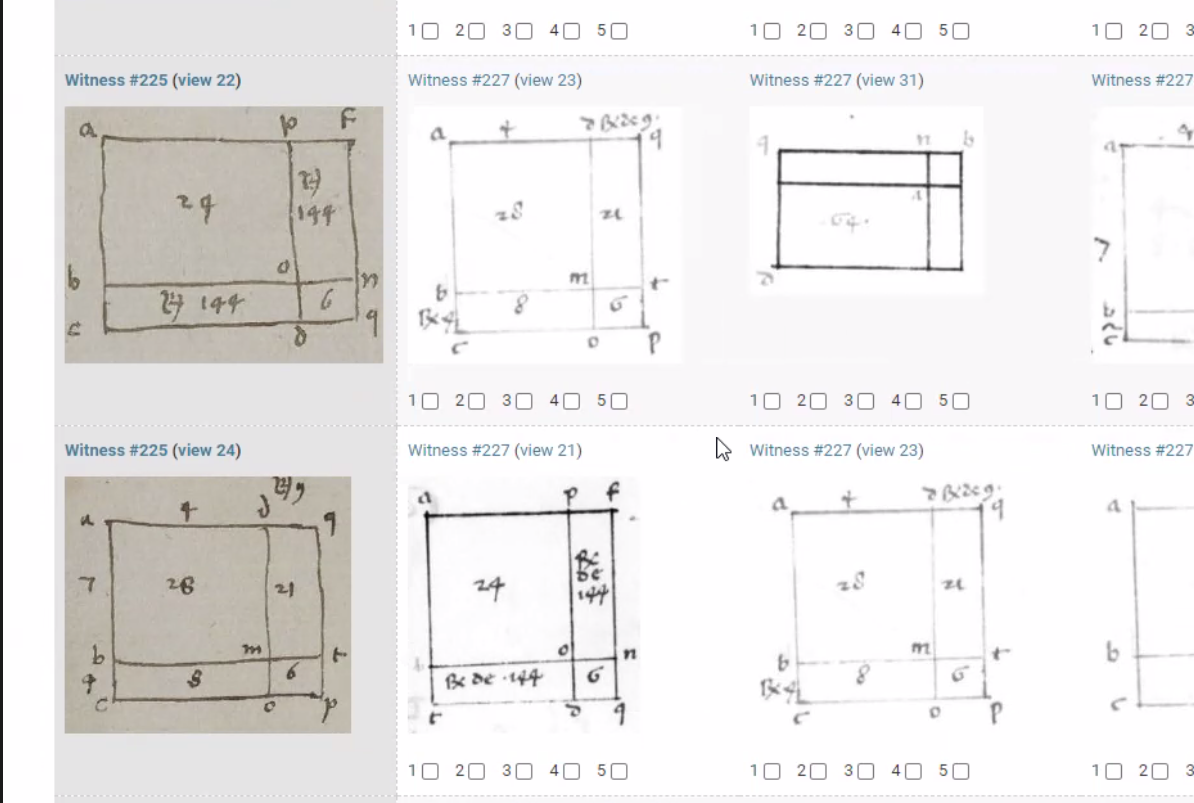
\includegraphics[height=7cm]{figues/label_dissim_exemple.png}
          \end{center}
          \caption{Impact des labels sur la recherche de similarité.}
          \label{fig:simlabel} \end{figure}

Devant ces difficultés il a été décidé d'adopter une annotation binaire
et basée uniquement sur le contenu graphique, partant du principe que
l'assignation d'un score de similarité par le modèle ne vaut pas pour
conclusion historiographique. Il sera toujours plus facile de ne pas
prendre en compte un résultat, et la visée de cet entraînement est
d'aboutir à un modèle assez extensif et généraliste. Il subsiste
cependant des dissensions au sein de l'équipe entre une définition très
stricte de la similarité, quitte à accepter des faux négatifs, et une
définition plus souple (typiquement, sensible aux labels), quitte à
créer des faux positifs. Pour concilier les besoins de tous les
chercheur.ses, il sera recommandé d'annoter selon la définition la plus
rigoureuse d'un point de vue scientifique, cette définition servant de
métadonnée aux chercheur.ses. Les annotations les plus souples seront
utilisées pour l'entraînement du modèle. Cette approche permet de
garantir une précision dans la classification des données tout en
offrant la souplesse nécessaire pour optimiser les performances des
algorithmes d'apprentissage automatique.

Ce cas d'étude est assez caractéristique des enjeux tenant à la
coordination au sein et entre des équipes de recherche dans le cadre du
développement d'un outil commun. D'où le développement des outils
d'annotation dans la plateforme commune assez généralistes pour que leur
usage s'adapte à des besoins différents et complexes\footnote{En
  réalité, les équipes de \vhs sont aussi passées à un classement binaire
  pour prévenir des problèmes de coordination au sein de leurs équipes,
  gardant l'usage des trois autres catégories pour une prochaine étape
  de fine-tuning.}.

\hypertarget{corpus}{%
\subsection{Corpus}\label{corpus}}

Les sources primaires d'\eida couvrent un spectre géographique et
temporel important. Orienté par les objectifs scientifique d'\eida --
arriver à une représentation globale des continuités et divergences qui
se tracent au cœur des pratiques astronomiques à travers l'histoire,
esquisser le voyage des sources à travers le temps et l'espace -- le
refus d'une vision eurocentrée justifie et explique une représentativité
large, servie par la constitution de cinq grands corpus issus de sphères
géographiques et temporelles diverses. Les manuscrits arabo-persans
produits entre le \textsc{viii}\ieme et le \textsc{xiii}\ieme siècle, des manuscrits latins
médiévaux produits majoritairement entre le \textsc{xiii}\ieme et le \textsc{xvi}\ieme siècle, les
manuscrits byzantins, produits entre les \textsc{ix}\ieme et \textsc{xv}\ieme siècles, les
manuscrits sanskrits, à partir du \textsc{xi}\ieme, et enfin les sources chinoises
datant du milieu du \textsc{xvi}\ieme siècle, après l'arrivée des premiers jésuites.
Le support de ces dernières n'est pas nécessairement le manuscrit, elles
prennent souvent la forme d'imprimés par blocs xylographiques dont les
matrices sont réemployées dans plusieurs témoins. Elles présentent donc
une forme hybride, sorte de pré-imprimé, qui posa des questions
complexes pour la modélisation conceptuelle des données.

Plusieurs centaines de manuscrits sont numérisés pour chaque tradition.
Sur ces numérisations, mises à disposition par les institutions
patrimoniales qui conservent ces témoins, seront appliquées les
traitements en prévision de l'analyse par les chercheur.ses, leur
permettant de souligner les motifs qui sous-tendent la diffusion
afro-eurasiens du modèle ptoléméen.

La gémellité avec \vhs impose un effort de modularité pour pouvoir
partager le modèle de données. Le travail de recherche de \vhs est mené
sur quatre corpus relevant, à l'instar de celui d'\eida d'une grande
diversité chronologique et géographique. Ces corpus se distinguent
cependant par une grande diversité thématique~: ils se composent de
manuscrits et d'imprimés concernant les sciences des mathématiques et
les sciences naturelles. Le premier corpus est le \emph{Physiologus},
rédigé vers le \textsc{ii}\ieme siècle à Alexandrie. Ce texte, l'un des plus
populaires du \ma, a contribué à l'émergence de la zoologie
chrétienne médiévale. Il a pour témoins 100 manuscrits grecs, dont treize
sont illustrés et réalisés entre le \textsc{xi}\ieme et le \textsc{xvi}\ieme siècle, contenant
environ 680 images d'animaux, de plantes et de minéraux. Le deuxième
corpus est le \emph{De materia medica} de Dioscoride, composé vers l'an
77 de notre ère. Ce traité pharmacologique destiné aux praticiens a été
largement diffusé et copié. Il est conservé dans 65 manuscrits grecs,
dont 17, réalisés entre le \textsc{vi}\ieme et le \textsc{xvi}\ieme{} siècle, sont illustrés et
contiennent environ 8340 images de plantes, d'animaux et de minéraux.
Les troisième et quatrième corpus se composent des planches de
l'Encyclopédie de Diderot et d'Alembert (1751-1772), les témoins de ce
travail couvrant une longue série de traités, dictionnaires et
encyclopédies au fil desquels les illustrations ont été copiées et
retravaillées. Leur étude se focalise aussi sur leur inclusion
ultérieure dans des encyclopédies telles que l'Encyclopédie méthodique.
Le troisième corpus se concentre sur l'Histoire naturelle (Zoologie),
tandis que le quatrième porte sur les sciences mathématiques\footcite{noauthor_vhs_nodate}.

Le deux corpus jumeaux diffèrent aussi en taille~: celui de \vhs présente plus de 2000 témoins devant 300 pour \eida.

Malgré ces divergences importantes, les données sont issus de spectres
assez larges pour opérer des croisements dont l'exploitation peut
s'avérer fructueuse~: les corpus \vhs présentent quelques diagrammes
astronomiques, et les manuscrits \eida présentent plusieurs images de
plantes. La mise en commun des résultats permet d'établir des liens
entre le \ma (focus d'\eida) et la période moderne (focus de \vhs)
pour les domaines respectifs étudiés. Notamment, des chercheur.ses d'\eida
s'intéressent à la transition du manuscrit à l'imprimé. La possible
jonction des corpus reste néanmoins problématique, et les modèles d'\ia doivent être spécialisés sur les objets d'étude respectifs des deux projets.

Ces remarques sont révélatrices de l'entre-deux qui nous intéresse dans
ce mémoire~: bien que les projets aient un objectif et des objets
d'étude précis, ceux-ci se trouvent élargis par le réseau institutionnel
et les dynamiques collaboratives qui accompagnent la création des outils
numériques. Le niveau de modularité de l'outil créé devra prendre en
compte cette généralisation possible sans perdre de vue les objectifs
initiaux des deux projets.

\hypertarget{modele-de-donnees}{%
\subsection{Modèle de données}\label{modele-de-donnees}}

L'application commune à \vhs/\eida est développée avec le \textit{framework} Django
et adossée sur une base de données gérée avec PostgreSQL. Le modèle de
données conçu pour l'application a fait l'objet de réflexions et
réadaptations pour répondre aux besoins de description des sources de
\vhs et \eida, tout en restant suffisamment flexible pour être utilisé par
d'autres projets souhaitant reproduire les méthodes employées par les
deux projets. Le défi consiste à conceptualiser la donnée de manière
suffisamment spécifique et assez généraliste.

\hypertarget{modele-initial}{%
\subsubsection{Modèle initial}\label{modele-initial}}

Le modèle de données initialement construit\footnote{Voir l'annexe \ref{data_models} pour une illustration de l'évolution du modèle de données.} pour
l'application \vhs prévoit l'existence des entités 'manuscrit' et
'imprimé', qui correspondent aux supports représentés dans
les corpus d'\eida et de \vhs. Ces deux \emph{états matériels} du texte
sont reliés à une entité plus abstraite~: le \wo.
S'appuyant sur la définition de \wo que donne le CIDOC-CRM\footnote{Le
  modèle conceptuel définit, dans un domaine donné, comment représenter
  la réalité. À ce titre il est indépendant de la manière dont on stocke
  les données informatiquement. Né dans le domaine des musées, CIDOC-CRM
  est un modèle conceptuel standardisé pour la modélisation des
  informations dans le domaine du patrimoine. Il vise à décrire et à
  rendre interopérables des objets du monde culturel en général. La
  notion d'événement se trouve au cœur du modèle, traduisant une
  approche monotonique des données~: les objets décrits peuvent évoluer,
  on peut toujours décrire de nouveaux événements liés à cet objet.
  Ainsi, on n'aura potentiellement jamais terminé de décrire un objet en
  CIDOC-CRM.}, un \wo est indépendant de sa forme matérielle, c'est une
production intellectuelle qui peut se manifester dans différentes
sources, pouvant elles-mêmes présenter des variations.

Mais ce premier modèle va rapidement montrer des limites, notamment
liées à la description d'une même œuvre divisée en plusieurs ouvrages,
ou d'un ouvrage contenant plusieurs œuvres. De plus, la pertinence de la
distinction absolue des manuscrits et imprimés ne permet pas une
description pertinente de tous les objets~: par exemple les sources
chinoises, dont le support n'est pas nécessairement le manuscrit,
prennent souvent la forme d'imprimés par blocs xylographiques dont les
matrices sont réemployée. Ces constats ont mené à la refonte de ce
modèle de données. 

\hypertarget{premiere-refonte}{%
\subsubsection{Première refonte}\label{premiere-refonte}}

Le nouveau modèle est non seulement plus pertinent mais aussi déjà plus
flexible. Il est centré autour de l'entité 'témoin' ou \wit, et
est complété par d'autre tables pour décrire la diversité des sources et
leurs différents modes d'existence. Ainsi, les séries héritent
uniquement des imprimés et les témoins héritent à la fois des
manuscrits et des imprimés. Une \ser est une édition en
plusieurs volumes d'une œuvre imprimée. Le témoin ramène à chaque volume
en tant qu'entité matérielle de référence, ou à un manuscrit. Il peut
contenir un ou plusieurs 'travaux' (\wo)~; un même \wo peut
correspondre à des séries et des témoins différents (table de relation
\textit{Content}). La table \wo inclut donc les références au lieu et à l'auteur
(clés étrangères), mais aussi l'information relative à la plage de temps
durant laquelle cette œuvre a existé physiquement (durant laquelle on
atteste l'existence de témoins). La ou les numérisations
(\digits) sont reliées au \wit et contiennent les détails sur la
source de numérisation et l'état des traitements via \iiif\footnote{Voir le \hyperlink{iiif}{Chapitre 2} sur \iiif}. Une entité Tag est utilisée comme moyen de
différencier manuscrit, imprimé ou gravure, et la table de relation
\textit{Tag\_Exemplar} fait le lien entre le témoin et les tags. La table
\textit{Role} établit des relations entre des contenus (\textit{Content}), des
\emph{séries} (\sers) et des personnes (\textit{Persons}), attribuant à
ces dernières les rôles d'auteur ou d'éditeur.

Les évolutions en cours pendant mon stage, détaillées en partie
III\footnote{Voir le \hyperlink{chapitre-7-processus-et-fonctionnalites}{Chapitre 7}}, ont nécessité de faire des choix
complexes, répondant à une double exigence \emph{a priori} paradoxale~:
une plus grande flexibilité pour intégrer de nouvelles sources de
données et une précision de description suffisante. De nouvelles
questions ont été soulevées liées à la granularité et à la cohérence
sémantique.

Ce paradoxe apparent met en lumière les défis et la complexité liés à la
modélisation de la donnée, et les transformations successives reflètent
des questionnements~: comment rendre l'application la plus universelle
possible, l'ouvrir à une large diversité de sources, sans renoncer à la
qualité de la description des sources des projets de \eida et \vhs~?
Comment, d'ailleurs, conceptualiser un modèle qui convienne aux deux
projets et leurs objectifs~? Les solutions ci-dessus décrites sont
satisfaisantes mais amenées à évoluer, montrant que la modularité se
construit sur le temps long.
                    
                \hypertarget{normalisation-donnees}{\section{%
                La normalisation des données d'annotation}\label{normalisation-donnees}}
                    \gaga mène une réflexion
méthodologique sur la portabilité des modèles, leur diffusion et le
partage de grands ensembles de données annotées selon des normes
communes. Les modèles d'\ia, notamment ceux dédiés à la
reconnaissance du texte manuscrit (\htr) et au traitement automatique des
langues (\tal), requièrent des données d'entraînement spécifiques. 

Mais si chaque projet de recherche annotait ses corpus selon ses propres
exigences, ils engendreraient fatalement des silos de données non
réutilisables. Pour garantir la réutilisation des données, il est
impératif d'établir des normes et des standards.

Le projet porte alors le développement d'une syntaxe
d'annotation générique pour harmoniser la segmentation des pages des
vérités de terrain, afin de constituer des corpus d'entraînement réutilisables. \gaga propose une
approche très inclusive en identifiant des éléments textuels communs à
une large variété de documents, manuscrits comme imprimés. Cette
démarche donne lieu à la définition d'un vocabulaire contrôlé permettant
ainsi de construire des corpus annotés compatibles avec différents contextes\footcite[``Using a common vocabulary to annotate zones called SegmOnto (that is still evolving), we have developed a generic workflow to analyse the layout, OCRise the text, and convert the ALTO output into minimally encoded TEI files (\dots).''][p.2]{janes_towards_2021}~:
SegmOnto\footnote{https://github.com/SegmOnto}

Les étapes de lemmatisation et d'étiquetage morphologique (POS-tagging) effectuées par les modèles de \tal sur le texte extrait des pages numérisées visent à normaliser le
langage en réduisant les mots à leur forme canonique (lemme) et en
identifiant leur catégorie grammaticale. Cette normalisation est
essentielle pour faciliter des analyses ultérieures telles que la
collation et la stylométrie. Elle permet une analyse comparative des textes
malgré la grande variabilité inhérentes aux
langues historiques, pour lesquelles l'absence de normes orthographiques entraîne une
grande diversité de graphies. La préparation des données, là aussi, a donné lieu à une
réflexion méthodologique sur les défis liés à la standardisation des
annotations linguistiques dans les corpus diachroniques.

Selon \citeauthor{gabay_standardizing_2020}~:
\begin{kwote}                     
	``With the development of big corpora of various periods, it becomes
	crucial to standardise linguistic annotation (e.g.~lemmas, POS tags,
	morphological annotation) to increase the interoperability of the data
	produced, despite diachronic variations.''\footcite[p.2]{gabay_standardizing_2020}
\end{kwote}  

\citeauthor{gabay_standardizing_2020}\footcite{gabay_standardizing_2020} relèvent la
difficulté de mettre en œuvre un cadre technique qui prenne en compte
les pratiques d'annotation déjà établies et propres à des états de la langue. Pourtant garantir une
interopérabilité minimale avec les corpus existants est essentielle pour
maximiser la valeur ajoutée des nouvelles données.

\begin{kwote}                     
	``Such a task cannot be done without taking into account longstanding
	annotation practices, in order to allow (minimal) interoperability with
	already existing datasets. Such a statement is sadly easier said than
	done, because EMF is an intermediary stage between medieval (12th-15th
	c.) and late modern and contemporary (from c.~1750) French, two states
	of language that tend to have different needs regarding annotation: EMF
	is then caught in between two (potentially incompatible) practices, one
	for each extreme of the continuum.''\footcite[p.2]{gabay_standardizing_2020}
\end{kwote}     

Il est particulièrement complexe de trouver un équilibre entre une
description linguistique trop fine, qui pourrait limiter
la réutilisabilité des corpus, et une description trop générale, qui pourrait
manquer de précision. De plus, les besoins en annotation varient considérablement
entre le français médiéval et le français moderne, et les systèmes
d'annotation de ses deux états de la langue sont difficilement
réconciliables~: or une large partie des sources de \gaga se
situent dans l'entre-deux. Trouver un compromis qui satisfait les
exigences spécifiques de chaque période est complexe.

L'harmonisation des annotations vise à favoriser la diffusion des corpus
de données sur HTR-United, une plateforme collaborative dédiée au
catalogage de vérités de terrain pour l'\htr et l'\ocr, principalement en
français\footcite{chague_htr-united_2021}. Cette base de
données, hébergée sur GitHub, centralise des images et leurs
transcriptions produites par différents projets de recherche, offrant
ainsi une diversité de jeux de données diachroniques et géographiques
pour l'entraînement de modèles \htr.

\gaga vise aussi à la diffusion des modèles en eux-même, qui peuvent alors être réutilisés et spécialisés. Par ailleurs, le projet
s'appuie sur des outils existants, par exemple Deucalion, une boîte à
outils de traitement automatique des langues (\tal) conçue pour être
interopérable avec d'autres systèmes\footnote{https://github.com/chartes/deucalion-model-af}.
                    

              


\vspace{2cm}


Les apports et les réflexions du projet \gaga reflètent la problématique globale de ce
mémoire~: comment concevoir des cadres pour l'environnement de la
recherche en Humanités Numériques, tout en répondant aux exigences
scientifiques de chaque projet. On voit se filer avec ce cas d'étude un écosystème complexe dans lequel s'agencent des systèmes et protocoles généraux et extensibles, adaptables aux besoins locaux, comme la \tei, ou SegmOnto, ou encore des \api pour la récupération des données. De nombreux défis restent cependant à relever, montrant que l'interopérabilité universelle est un idéal difficilement atteignable.

L'utilisation de l'\ia porte la question du partage des ressources à un niveau d'importance supérieur, puisque les modèles peuvent être spécialisés, et les corpus enrichis produits peuvent constituer des données d'entraînement. L'intervention du chercheur.se pour corriger les résultats des traitements automatiques est donc un aspect important à prendre en compte pour assurer la fiabilité scientifique de ses corpus annotés. 

\gaga visait à l'élaboration d'un
outil d'acquisition et d'enrichissement des données capable de se
détacher d'un corpus spécifique et sur ce point se voulait preuve de concept, mais le projet
n'a pas pleinement atteint ses objectifs, car la chaîne de traitement est restée très orientée vers les corpus de la \bnf. Il a ainsi mis en
évidence la complexité de concilier les exigences d'une infrastructure
générique et les besoins spécifiques des données, montrant que la modularité s'inscrit avant tout dans le temps. 

Comme le montre le cas de e-Scriptorium, une chaîne de traitement, si elle est assez généraliste pour tolérer une grande diversité de données, participe à la cohérence des pratiques et à la mutualisation des outils de la recherche. Les modalités d'accès (\textit{notebooks}, plateforme, scripts etc.) impactent la prise en main et l'adoption des outils. 

Plus généralement, les recherches menées sur l'enrichissement et l'exploration de larges corpus grâce aux outils d'\ia ouvrent de nouvelles perspectives en terme de trouvabilité et de fouille de données visuelles ou textuelles. Cette valeur ajoutée est liée au passage du format \jpeg à des formats balisés et sémantiquement riche qui permettent des exploitations ou l'indexation. 